\chapter{Motivación y Contexto}

La fotónica es una ciencia que utilizamos diariamente, por ejemplo, mediante los cables ópticos.
Los principales beneficios que ofrece son (i) elevado ancho de banda en comunicaciones, (ii) bajo consumo energético, (iii) interconexiones ópticas independientes de la distancia \citep{Glick2018}.
El potencial de la fotónica se logra evidenciar en aplicaciones que aprovechan estos beneficios; por ejemplo,
(i) interconexiones ópticas en centrales de datos \citep{Shen2019}, 
(ii) redes neuronales ópticas \citep{Shen2017}, 
(iii) internet de las cosas \citep{Glick2018}.


La importancia de estas aplicaciones en computación se evidencia aún más en la computación de alto rendimiento (HPC).
Un problema presentado en el Top500 sistemas HPC es que desde el año 2010, el ratio entre el ancho de banda entre nodos y el poder de procesamiento por nodo ($byte / FLOP$) ha decrecido en un factor de seis.
Así, se está llegando a un punto donde la capacidad para interconectar nodos está limitando el desempeño de sistemas HPC en programas que hacen uso extensivo de transferencias de memoria.
Ante este problema se han propuesto arquitecturas que aprovechan la transmitancia óptica porque esta puede realizar interconexiones a distancias del orden de metros. 
De esta manera se logra la transferencia de grandes cantidades de información con un bajo consumo energético y manteniendo un elevado ancho de banda \citep{Shen2019, Anderson2018}.


Las aplicaciones señaladas anteriormente demuestran el potencial de la fotónica, mas estas aún no logran ponerse en práctica. 
Para que cada una de ellas funcione se necesita fabricar chips de fotónica integrada con una elevada eficiencia y densidad.
Pero los diseños actuales aún son muy ineficientes por lo cual sigue conviniendo utilizar dispositivos electrónicos \citep{Glick2018, Vuckovic2019}. 
Ante esta dificultad, la fotónica en silicio (SiP) se presenta como un buen candidato para fabricar estos chips.
La idea se refuerza por la adaptación de procesos de semiconductor complementario de óxido metálico (CMOS) para fabricar dispositivos SiP.
Esto es un gran beneficio porque los procesos CMOS son una tecnología bien establecida y con precios accesibles \citep{Glick2018, Shen2019, LukasChrostowski2010}.


Por estos motivos, una cantidad considerable de investigaciones estudian dispositivos SiP \citep{Molesky2018}.
El presente trabajo se centrará en dos de ellos: \emph{bend-90°} y \emph{wavelength demultiplexer} de dos canales.
De aquí en adelante nos referiremos a estos simplemente como \emph{bend} y WDM, respectivamente.


El documento está organizado de la siguiente manera:

El capítulo 1 brinda una introducción al tema de investigación, describe el problema a detalle, justifica la relevancia de resolverlo, define los objetivos y señala los aportes del trabajo.

El capítulo 2 desarrolla conceptos fundamentales en fotónica necesarios para entender el resto del documento.

El capítulo 3 presenta una revisión del estado del arte y discute sus principales características.

El capítulo 4 expone la metodología usada en la investigación.

El capítulo 5 muestra los resultados preliminares obtenidos con los experimentos.

\section{Introducción}

La fotónica está atrayendo el interés de la industria debido a su potencial en términos de escalabilidad y los beneficios de costo-eficiencia. 
Este potencial es evidente, por ejemplo, con los siguientes tres puntos. 
Primero, si se quiere mantener la tendencia que cada 10 años se mejore en un factor de 1000 el rendimiento de los sistemas electrónicos, entonces parece ser indispensable la convergencia de estos con sistemas fotónicos \citep{Glick2018}. 
Segundo, existe una inversión billonaria en la fabricación de transistores cuyos procesos se están adaptando para fabricar chips de fotónica integrada \citep{LukasChrostowski2010}.
Tercero, hay prometedoras aplicaciones en (i) interconexiones ópticas \citep{Shen2019}, (ii) redes neuronales ópticas \citep{Shen2017}, (iii) internet de las cosas \citep{Glick2018}.
 

SiP se está estudiando con el fin de mostrar el potencial de la fotónica, pero esta tecnología aún se encuentra en la misma etapa de expansión que tenía la electrónica en los años 1970s.
Afortunadamente, ya existen \emph{foundries} y procesos como el CMOS que se pueden emplear como infraestructura para la fabricación de chips SiP \citep{LukasChrostowski2010}.
Pero, los chips SiP siguen siendo ineficientes por lo cual se está buscando optimizar dispositivos fundamentales que lo componen \citep{Vuckovic2019}.
Para esto existen dos estrategias: diseño tradicional y diseño inverso.


En el diseño tradicional se define el dispositivo con geometrías simples que permiten obtener funciones analíticas de sus propiedades físicas \citep{Hughes2016, Song2008}. 
Esto se realiza para poder optimizar la función obtenida a partir de los parámetros que la definan. 
Dicha optimización se suele ejecutar haciendo un barrido de los parámetros, con algoritmos genéticos o usando \emph{particle swarm optimization}. 
Es un enfoque simple, pero que ha obtenido buenos resultados. 
Sin embargo, existen tres grandes inconvenientes con este planteamiento. 
Primero, solo estamos explorando una pequeña fracción de todos los posibles diseños.
Segundo, por lo general no es conocido el límite de rendimiento del dispositivo.
Tercero, al trabajar en la escala de nanómetros, existen casos como el \emph{bend} y WDM que presentan un bajo rendimiento con diseños tradicionales \citep{Molesky2018, Su2020}.


En el diseño inverso se busca hacer una mayor exploración de todos los posibles diseños. 
Para ello, ya no nos limitamos a solo usar diseños intuitivos, ver figura \ref{fig:devices}. 
Ahora, definimos geometrías arbitrarias y usamos simulaciones computacionales para determinar las propiedades físicas del dispositivo \citep{Molesky2018, Su2020}. 
Este enfoque ha logrado conseguir mejores resultados que los obtenidos por el diseño tradicional \citep{Su2018, Molesky2018}. 
Sin embargo, este planteamiento viene acompañado de nuevos desafíos.


\begin{figure}[ht]
  \centering
  % 1° row
  % Traditional bend
  \subfigure[\emph{Bend} con diseño tradicional]{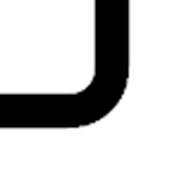
\includegraphics[width=0.4\textwidth]{image/introduction/traditional-bend.png}}
  \hfill
  % Inverse design bend
  \subfigure[\emph{Bend} obtenido con diseño inverso. Extraído de \citep{Su2020}]{
    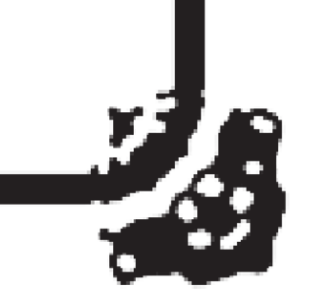
\includegraphics[width=0.4\textwidth]{image/introduction/inverse-design-bend.png}
  }

  % 2° row
  % Traditional splitter
  \subfigure[WDM con diseño tradicional]{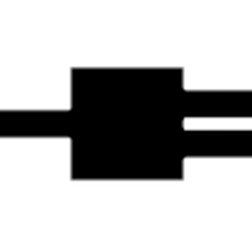
\includegraphics[width=0.4\textwidth]{image/introduction/traditional-splitter.png}}
  \hfill
  % Inverse design splitter
  \subfigure[WDM obtenido con diseño inverso. Extraído de \citep{Su2020}]{
    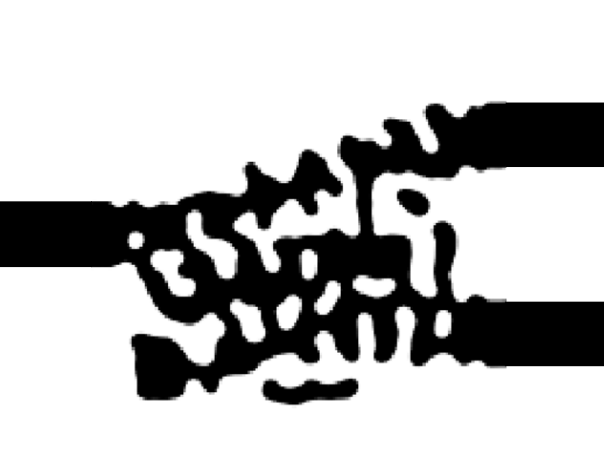
\includegraphics[width=0.4\textwidth]{image/introduction/inverse-design-splitter.png}
  }

  \caption{Diseños tradicionales y obtenidos a partir de diseño inverso de un \emph{bend} y un WDM}
  \label{fig:devices}

\end{figure}


El diseño inverso ha recibido mucha atención en fotónica durante los últimos 20 años \citep{Molesky2018}. 
Los autores en \cite{Su2020} muestran estrategias para optimizar un \emph{bend} y \emph{WDM}.
En \cite{Su2018, Piggott2017} se incorporan restricciones de fabricación para obtener dispositivos que al fabricarse mantengan un buen rendimiento. 
No obstante, la búsqueda de estos diseños suele realizarse aplicando algoritmos cuya selección y configuración es mayormente debido a un tedioso proceso de prueba y error.
Otros trabajos como los de \cite{Schneider2019, Elsawy2020, Gregory2015} comparan distintos algoritmos de optimización en el diseño inverso de dispositivos fotónicos.


Aún cuando una cantidad considerable de investigaciones están usando el diseño inverso para optimizar dispositivos fotónicos, el \emph{bend} y WDM, dispositivos fundamentales para los circuitos fotónicos, aún no logran aplicación comercial \citep{Molesky2018}.
Además, existe una carencia de estudios con un enfoque computacional que intenten abordar el problema.
Asi, el objetivo de esta tesis es aplicar el conocimiento en computación para optimizar estos dispositivos y conseguir diseños que al fabricarse muestren un desempeño elevado.


\section{Descripción del Problema}


Para poder describir el funcionamiento de un dispositivo se calcula la distribución del campo eléctrico, para ello se resuelven las ecuaciones
de Maxwell \citep{Schneider2019}. 
Una forma de encontrar la solución a estas ecuaciones en cualquier geometría es utilizando un método numérico llamado diferencias finitas en el dominio de frecuencias (FDFD) \citep{Su2020}.
Con este planteamiento se selecciona una región rectangular a optimizar y se la divide  en $n \times m$  píxeles como si fuera una imagen, ver Figura \ref{fig:bend-discretization}. 
Luego, cada píxel se rellena con dos posibles materiales: óxido de silicio ($SiO_2$) o silicio ($Si$) \citep{Molesky2018}.

\begin{figure}[ht]
  \centering
  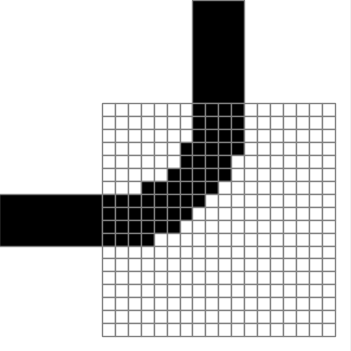
\includegraphics[scale=0.6]{image/introduction/bend-discretization.png}
  \caption{\emph{Bend} con una región de diseño discretizada en $18 \times 18$ píxeles. Cada píxel negro representa la presencia de $Si$ y cada píxel blanco de $SiO_2$}
  \label{fig:bend-discretization}
\end{figure}

El diseño inverso comienza definiendo los requerimientos del dispositivo para luego tratar de buscar entre los $2^{n \times m}$ posibles diseños algún candidato que se adapte a lo que se busca \citep{Su2020, Molesky2018}.
Como prueba de concepto, trabajos como el de \cite{Malheiros-Silveira2020} parametrizaron $2^{10 \times 10}$ posibles geometrías.
Así, se presentan algunas dificultades con esta estrategia:

\begin{enumerate}
  \item No es viable evaluar todos los posibles diseños por haber un número excesivamente elevado de ellos \citep{Vuckovic2019}.
  \item Las simulaciones computacionales son muy costosas en términos de memoria y tiempo \citep{Kudyshev2020}.
  \item El espacio de búsqueda es no convexo \citep{Su2018}.
  \item No todos los diseños son fabricables por limitaciones físicas \citep{Su2020}.
  \item Cada dispositivo es una clase distinta de problema, es decir, no necesariamente funcionará la misma estrategia para cada dispositivo \citep{Molesky2018}.
\end{enumerate}

Además, la fabricación viene con otros desafíos, principalmente:

\begin{enumerate}
  \item Errores de precisión \citep{Piggott2017}.
  \item Sensibilidad ante cambios de temperatura \citep{Vuckovic2019}.
\end{enumerate}

Considerando las anteriores dificultades, el problema es usar diseño inverso y encontrar geometrías que muestren buen desempeño en simulaciones computacionales y que puedan asegurar mantener un óptimo funcionamiento al ser fabricados. 
Este problema se estudiará para dos dispositivos nanofotónicos (i) \emph{bend} y (ii) WDM.

\section{Justificación}

El \emph{bend} y WDM son dispositivos fundamentales en los circuitos fotónicos que tienen aplicación directa, por ejemplo, en sistemas HPC \citep{Shen2017}. 
Por otro lado, desde el punto de vista computacional, este problema es interesante porque ya hay estrategias computacionales conocidas para resolverlo, desde algoritmos evolutivos \citep{Hansen2016} hasta redes neuronales \citep{Goodfellow2015} y \emph{depth learning} \citep{Malkiel2018}. 
Además, debido al alto costo computacional de las simulaciones \citep{Schneider2019}, el trabajo requiere de computación de alto desempeño.
Así, es probable que se pueda obtener buenos resultados en la investigación aplicando el conocimiento ya existente en computación. 

\section{Objetivos}

\begin{itemize}

  \item Fabricar un \emph{bend} y WDM con eficiencias mayores al noventa por ciento.

  \begin{itemize}

    \item Encontrar geometrías que muestren esta característica en simulaciones computacionales

    \item Encontrar geometrías resilientes a posibles errores de fabricación de dilatación o contracción

  \end{itemize}

  \item Usando HPC, estudiar el desempeño y la convergencia de cinco algoritmos de optimización populares usados para optimizar dispositivos nanofotónicos.

\end{itemize}



\section{Aportes}

Este trabajo busca brindar una comparativa de las técnicas de optimización más relevantes que se aplican para optimizar un \emph{bend} y un WDM cuando estos son parametrizados con un elevado número de variables.

%\joruge{por ahora mantener, luego alinear al paper de JLT}
